\documentclass[10pt,a4paper]{article}


% --- Encodage et langue ---
\usepackage[utf8]{inputenc}
\usepackage[T1]{fontenc}
\usepackage[french]{babel}

% --- Mise en page ---
\usepackage[top=2.1cm, bottom=1.8cm, left=1.8cm, right=1.8cm]{geometry}
\usepackage{setspace}
\singlespacing

% --- Images ---
\usepackage{graphicx}
\usepackage{float}
\usepackage{subcaption}  % pour les sous-figures côte à côte

% --- Mathématiques ---
\usepackage{amsmath}

% --- Liens et couleurs ---
\usepackage{hyperref}
\usepackage{xcolor}

% --- Divers ---
\usepackage{enumitem}     % listes compactes
\usepackage{parskip}      % espace entre paragraphes au lieu d'indentation
\usepackage{microtype}    % meilleure justification
% Réduire l'espace autour des titres de section
\usepackage{fancyhdr}

% Pas de numérotation de page (optionnel)
% \pagestyle{empty}
\setlength{\parindent}{0pt}
\setlength{\parskip}{0.35em}
\pagestyle{fancy}
\fancyhf{}
\lhead{Victor Henri Willy Eder\\Liam Van Camp}
\rhead{27 mars 2026\\EPFL Microtechnique}
\renewcommand{\headrulewidth}{0pt}
\setlength{\headheight}{28pt}
\setlength{\headsep}{18pt}

\begin{document}
\begin{center}
    {\huge \textbf{Rapport d'activit\'e -- Rendu 3}}
\end{center}
\vspace{0.5cm}

% ============================================================
\section*{Partie 1 — Dynamiques du jeu}
% ============================================================

% ------------------------------------------------------------
\subsection*{1.1 Changements structurels par rapport au Rendu 2 (optionnel)}
% ------------------------------------------------------------

% Listez ici les modifications apportées aux structures de données
% ou algorithmes. Si rien n'a changé, supprimez cette sous-section.

\begin{itemize}[noitemsep, topsep=2pt]
    \item \texttt{Ball} : ajout des méthodes \texttt{translate()} et
      \texttt{setDelta()} pour rendre la classe mutable.
    \item \texttt{Paddle} : ajout de l'attribut \texttt{last\_delta}
      et de la méthode \texttt{getDelta()} pour la collision
      balle-raquette.
    \item \texttt{Brick} : ajout de la méthode virtuelle pure
      \texttt{hit()} dans la hiérarchie de classes.
    \item \texttt{Game} : réécriture complète de \texttt{update()}
      avec les trois phases de la dynamique.
    % Ajoutez ou supprimez des points selon vos vrais changements
\end{itemize}

% ------------------------------------------------------------
\subsection*{1.2 Collision de deux balles de rayons diff\'{e}rents}
% ------------------------------------------------------------

\noindent
\begin{minipage}[t]{0.50\textwidth}
La balle $A$ (petite, rayon $r_a$) se d\'{e}place et entre en
contact avec la balle $B$ (grande, rayon $r_b$). La collision est
d\'{e}tect\'{e}e d\`{e}s que la distance entre leurs centres est
inf\'{e}rieure \`{a} $r_a + r_b + \epsilon$.

\medskip
Lors de l'impact, les deux balles rebondissent~: une impulsion est
appliqu\'{e}e le long de l'axe reliant leurs centres,
pond\'{e}r\'{e}e par le rapport des rayons. Les composantes
tangentielles restent inchang\'{e}es et les normes des deltas sont
born\'{e}es \`{a} \texttt{delta\_norm\_max}.
\end{minipage}%
\hfill
\begin{minipage}[t]{0.45\textwidth}
\vspace{-15pt}
\centering
\begin{minipage}[t]{0.20\linewidth}
\centering
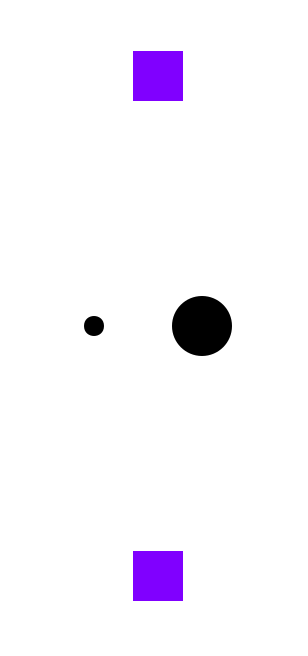
\includegraphics[width=\linewidth]{photo_rapport_3/B1.png}\\[2pt]
{\small\hspace{25pt} Avant}
\end{minipage}\hfill
\begin{minipage}[t]{0.21\linewidth}
\centering
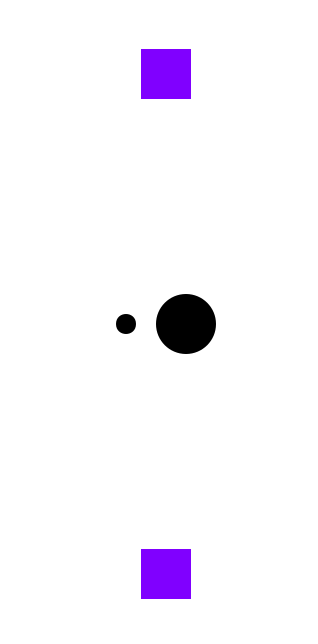
\includegraphics[width=\linewidth]{photo_rapport_3/B2.png}\\[2pt]
{\small\hspace{25pt} Avant}
\end{minipage}\hfill
\begin{minipage}[t]{0.215\linewidth}
\centering
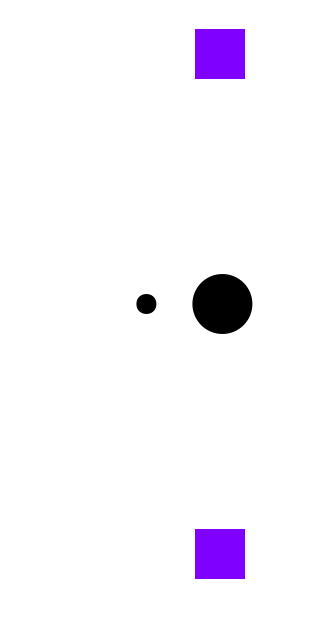
\includegraphics[width=\linewidth]{photo_rapport_3/B3.png}\\[2pt]
{\small\hspace{27pt} Apr\`{e}s}
\end{minipage}\hfill
\begin{minipage}[t]{0.25\linewidth}
\centering
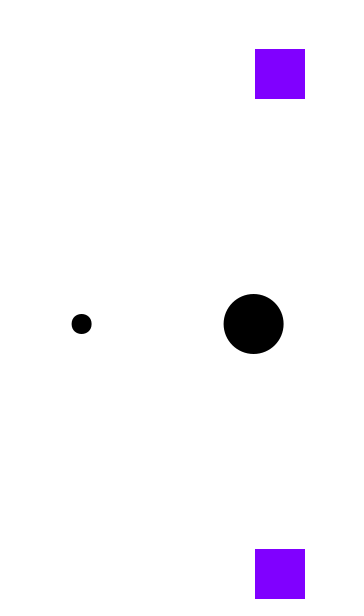
\includegraphics[width=\linewidth]{photo_rapport_3/B4.png}\\[2pt]
\vspace{10pt}
{\small\hspace{1pt} Apr\`{e}s}
\end{minipage}

\captionsetup{hypcap=false}%
\end{minipage}
\vspace{0.5cm}
% ------------------------------------------------------------
\subsection*{1.3 Destruction de chaque type de brique}
% ------------------------------------------------------------

% --- Ligne 1 : RainbowBrick ---
\noindent
\begin{minipage}[t]{0.60\textwidth}
\textbf{RainbowBrick} : \`{a} chaque impact, la brique perd
1 \texttt{hit\_point} et sa couleur change. Elle est
d\'{e}truite lorsque ses points de vie atteignent z\'{e}ro.
\end{minipage}\hfill
\begin{minipage}[t]{0.30\textwidth}
\makebox[1.2em][l]{\small(a)}%

\includegraphics[width=0.91\linewidth]{photo_rapport_3/rb1.png}%
\\[2pt]
\makebox[1.2em][l]{\small(b)}%

\includegraphics[width=0.91\linewidth]{photo_rapport_3/rb2.png}%
\\[2pt]
\makebox[1.2em][l]{\small(c)}%

\includegraphics[width=0.91\linewidth]{photo_rapport_3/rb3.png}
\end{minipage}

\medskip
% --- Ligne 2 : BallBrick ---
\noindent
\begin{minipage}[t]{0.38\textwidth}
\textbf{BallBrick} : d\'{e}truite d\`{e}s le premier impact.
Une nouvelle balle est g\'{e}n\'{e}r\'{e}e au centre de la
brique, h\'{e}ritant du delta incident de la balle frappante.
\end{minipage}\hfill
\begin{minipage}[t]{0.58\textwidth}
\begin{minipage}[t]{0.30\linewidth}
\centering

\includegraphics[width=\linewidth]{photo_rapport_3/bb1.png}
\end{minipage}\hfill
\begin{minipage}[t]{0.30\linewidth}
\centering

\includegraphics[width=\linewidth]{photo_rapport_3/bb2.png}
\end{minipage}\\[2pt]
\begin{minipage}[t]{0.30\linewidth}
\centering

\includegraphics[width=\linewidth]{photo_rapport_3/bb3.png}
\end{minipage}\hfill
\begin{minipage}[t]{0.30\linewidth}
\centering

\includegraphics[width=\linewidth]{photo_rapport_3/bb4.png}
\end{minipage}
\end{minipage}

\medskip
% --- Ligne 3 : SplitBrick ---
\noindent
\begin{minipage}[t]{0.38\textwidth}
\textbf{SplitBrick} : d\'{e}truite au premier impact. Elle
spawne 4 briques filles de taille
$(\text{size} - \texttt{split\_brick\_gap})/2$,
uniquement si cette taille $\geq$ \texttt{brick\_size\_min}.
\end{minipage}\hfill
\begin{minipage}[t]{0.58\textwidth}
\makebox[1.2em][l]{\small(a)}%
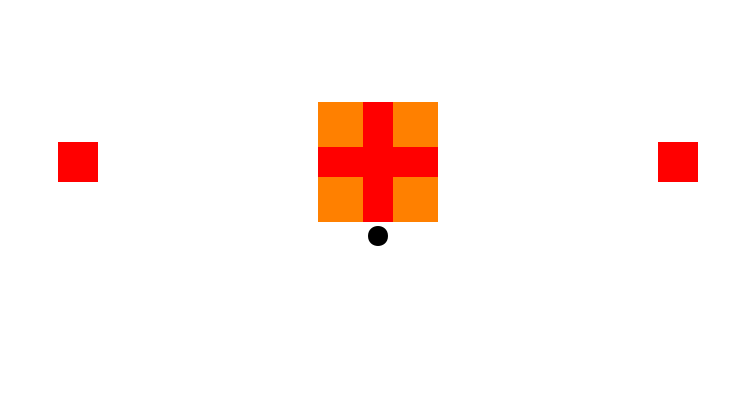
\includegraphics[width=0.91\linewidth]{photo_rapport_3/sb1.png}%
\\[2pt]
\makebox[1.2em][l]{\small(b)}%

\includegraphics[width=0.91\linewidth]{photo_rapport_3/sb2.png}%
\\[2pt]
\makebox[1.2em][l]{\small(c)}%

\includegraphics[width=0.91\linewidth]{photo_rapport_3/sb3.png}
\end{minipage}

\newpage  % ← Force le passage à la page 2

% ============================================================
\section*{Partie 2 — Travail en groupe et bilan}
% ============================================================

% ------------------------------------------------------------
\subsection*{2.1 Activité individuelle}
% ------------------------------------------------------------

\begin{itemize}[noitemsep, topsep=2pt]
    \item \textbf{Liam Van Camp :} \textit{[Décrivez votre
      contribution — modules, fonctions, tests, etc.]}
    \item \textbf{Victor Eder :} \textit{[Décrivez sa contribution
      — modules, fonctions, tests, etc.]}
\end{itemize}

% ------------------------------------------------------------
\subsection*{2.2 Méthodologie}
% ------------------------------------------------------------

\textbf{Organisation et outils :}
\textit{[Décrivez comment vous vous êtes organisés — Git (branches,
commits), VSCode Live Share, réunions, etc.]}

\textbf{Ordre de développement et tests :}
\textit{[Dans quel ordre avez-vous développé les modules ? Ex :
tools → ball/brick/paddle → game::load → game::update. Quelles
méthodes de test pour chaque partie (fichiers .txt manuels,
débogage visuel, etc.) ?]}

\textbf{Travail simultané vs indépendant :}
\textit{[Quelle proportion du code a été écrite côte à côte (pair
programming) vs en parallèle de façon indépendante ? Avec le
recul, changeriez-vous cette proportion, et pourquoi ?]}

% ------------------------------------------------------------
\subsection*{2.3 Bug le plus fréquent}
% ------------------------------------------------------------

\textit{[Décrivez le bug qui revenait le plus souvent — ex : balle
traversant les briques (effet tunnel), boucle infinie dans
update(), mauvaise direction nominale, etc. Quelle était la cause,
comment l'avez-vous détecté et résolu ?]}

% ------------------------------------------------------------
\subsection*{2.4 Usage d'un outil d'IA}
% ------------------------------------------------------------

\textit{[Avez-vous utilisé un outil d'IA (Claude, ChatGPT,
Copilot, etc.) ? Si oui, pour quelles tâches (compréhension des
formules de collision, débogage, structuration du rapport, etc.) ?
Gain ou perte de temps — quantifiez approximativement (ex :
``gain d'environ 1h sur la compréhension de la formule
d'impulsion balle-balle'').]}

% ------------------------------------------------------------
\subsection*{2.5 Conclusion}
% ------------------------------------------------------------

\textit{[Auto-évaluation courte sur deux axes :]}

\textbf{Code :} \textit{[Robustesse (gestion des cas limites,
boucles infinies évitées via nb\_bounce\_max, etc.) et performance
(complexité des boucles dans update(), etc.)]}

\textbf{Environnement de travail :} \textit{[Points forts et
points faibles de l'environnement fourni (GTKmm, structure
imposée, fichiers de test, etc.) et améliorations que vous
suggéreriez.]}

% ============================================================
\end{document}
% ============================================================
